\subsection{System Call Invocation Frequencies}
To determine what calls we should test, we used strace and ltrace to monitor library and system calls, respectively. We ran calls on small command-line utilities that we felt represented a realistic workload, given in tables \ref{lst:coreutils}, \ref{lst:net-tools}, and \ref{lst:other_utilities}. Histograms of the system call counts and library call counts are shown in figures \ref{fig:sys_counts} and \ref{fig:lib_counts}, respectively. We were unable to test some calls because they did not return any value (e.g. free). Other frequently made calls were discarded because they were not conducive to library interposition. Finally, still others were we felt were unlikely to be called by application code. \\
\begin{figure}
\centering
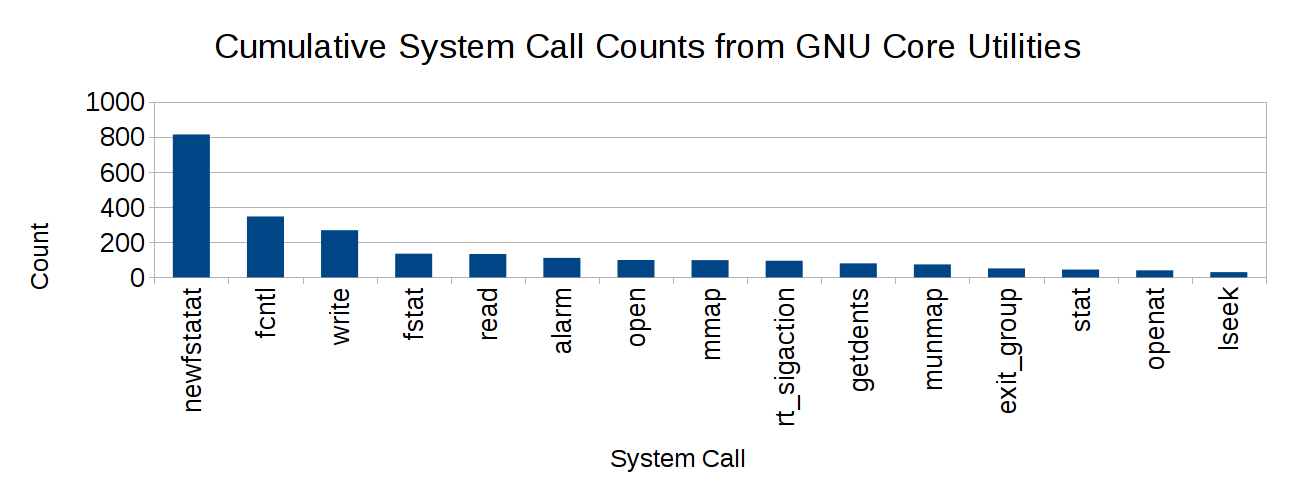
\includegraphics[width=\textwidth]{sys_counts}
\caption{Most frequently invoked system calls in a sample run of common utilities}
\label{fig:sys_counts}
\end{figure}

\begin{figure}
\centering
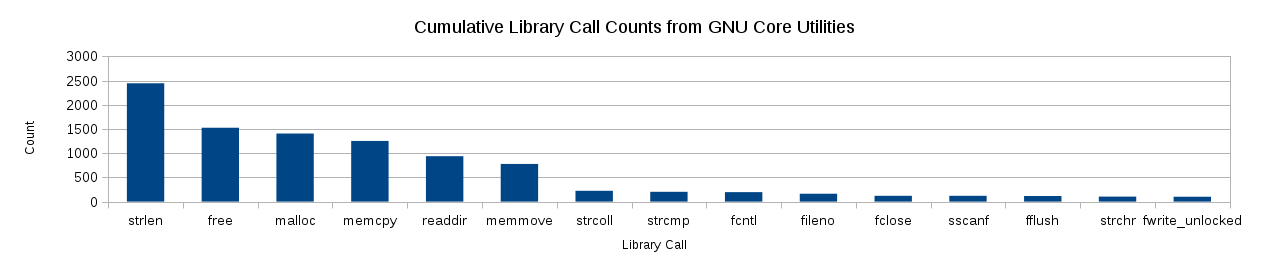
\includegraphics[width=\textwidth]{lib_counts}
\caption{Most frequently invoked library calls in a sample run of common utilities}
\label{fig:lib_counts}
\end{figure}
